% ======================================================================
% QIJ — WSOM+2026 submission draft, v4
% Abstract + Sec 1 = author-edited (banked via chat); Secs 2-5 = Claude
% draft aligned to the banked vocabulary, awaiting author pass.
%
% TERMINOLOGY REGISTRY (current)
%   X = {x_i in R^d}, i=1..N   — dataset, sample size N
%   \hat F                     — empirical distribution of the sample
%   psi                        — influence function (defined Sec 2.1)
%   RF                         — receptive field (defined Sec 2.1);
%                                never bare "cell" or "field"
%   W, w_j, j                  — prototype set / prototype / RF index
%   n_j, p_j = n_j/N, p        — RF counts, mass fractions, vector
%   T(p)                       — estimator as function of mass fractions
%   V_tot = V_btw + V_win      — macros \Vtotal \Vcell \Vwithin
%   em dashes                  — only where the author wrote them;
%                                otherwise ", explanation" format
%   \todo{..}                  — awaiting runs or author confirmation
%
% OPEN ITEMS FROM SEC-1 EDITING (flagged, easy to revert):
%   [A] Intro decomposition para: I inserted the 5-word clause
%       "QIJ measures the first directly, and recovers the second from the same partition statistics." (recommended, not yet
%       explicitly approved) — delete the sentence to revert.
%   [B] The 22%-coverage empirical sentence remains OUT of Sec 1
%       (author rewrite omitted it; restoration was offered, no reply).
% ======================================================================
\documentclass[runningheads]{llncs}

\usepackage[T1]{fontenc}
\usepackage{graphicx}
\usepackage{amsmath,amssymb}
\usepackage{mathtools}
\usepackage{url}
\usepackage{booktabs}
\usepackage{xcolor}

% --- draft machinery (delete before submission) ---
\newcommand{\todo}[1]{\textcolor{red}{[TODO: #1]}}
\newcommand{\placeholderfig}[2]{%
  \fbox{\parbox[c][#1][c]{0.94\linewidth}{\centering\ttfamily\small #2}}}

% --- notation ---
\newcommand{\ifl}{\psi}
\newcommand{\Vcell}{V_{\mathrm{btw}}}
\newcommand{\Vwithin}{V_{\mathrm{win}}}
\newcommand{\Vtotal}{V_{\mathrm{tot}}}
\newcommand{\Fhat}{\hat F}

\begin{document}

\title{Vector Quantization for Uncertainty Quantification: The Quantized Infinitesimal Jackknife}

\titlerunning{Vector Quantization for Uncertainty Quantification}
% ORCID iDs can be added via \orcidID{...} after each name if desired
\author{Josh Taylor\inst{1}\thanks{Corresponding author.} \and
Stella S. R. Offner\inst{1}}
\authorrunning{J. Taylor and S. S. R. Offner}
\institute{The University of Texas at Austin, Department of Astronomy and Oden Institute for Computational Engineering and Sciences, Austin, Texas, USA
\email{joshtaylor@utexas.edu}}

\maketitle

\begin{abstract}
Nonparametric confidence intervals (CIs) for a parameter estimate $T(X)$ are commonly obtained by the bootstrap: recompute $T(X_b)$ on $B$ resampled datasets $X_b$ and infer estimate uncertainty from the replicates. The bootstrap is the gold standard, but it costs $B$ evaluations of the estimator, prohibitive when a single fit is expensive, e.g.\ when $T$ must be found by numerical optimization rather than in closed form. We show that a fitted vector quantizer offers a much cheaper route to the same intervals. The Quantized Infinitesimal Jackknife (QIJ) uses the quantizer's $M$ receptive fields (with counts $n_j$) as the variables of the uncertainty calculation: the estimator is re-expressed as a function of the counts, and QIJ measures how $T(X)$ responds when each $n_j$ is perturbed, which is the natural impact of resampling on a VQ. This requires only $M{+}1$ evaluations of $T(X)$ in total, vs.\ $B \gg M{+}1$ in the standard bootstrap. We infer the variance and skewness of the estimate by propagating the counts' exactly known (multinomial) sampling fluctuations through the measured responses; both feed our VQ-enabled CIs, and no resampling occurs anywhere. On two synthetic distributions (Pareto; multivariate $t$ in ten dimensions) and an astronomical dataset (the galaxy fundamental plane), QIJ matches the bootstrap's coverage and interval widths at a small fraction of its computation.
\keywords{vector quantization \and uncertainty quantification \and confidence intervals \and influence functions \and bootstrap}
\end{abstract}


% ======================================================================
\section{Introduction}\label{sec:intro}
% ======================================================================

Vector quantization (VQ) compresses a dataset $X = \{x_i \in \mathbb{R}^d\}_{i=1}^N$ into $M \ll N$ prototypes $W = \{w_j\}_{j=1}^M$ to facilitate signal encoding, clustering, density representation \cite{graf2000}, and, through self-organizing maps and their descendants, topology-preserving visualizations. In this work, we assign VQ a different task in the statistical inference domain: constructing confidence intervals for an arbitrary estimator computed from $X$.

The bootstrap \cite{efron1979} is the gold standard for nonparametric interval estimation: recompute the estimator $T$ on $B$ resampled datasets, with $B$ in the hundreds to thousands, and infer CIs from the replicated sampling distribution of $T(X)$. When a single evaluation of $T$ is expensive, e.g., the result of an optimizer-based fit, a profile likelihood, or an ensemble, those $B$ evaluations dominate the analysis. VQs represent large data well; it is natural to assume data prototypes (learned by the VQ) could stand in for the $N$ sample points during resampling. This works well for point estimates, but not for interval estimation. That is, in terms of uncertainty quantification, the quantizer prototypes are not just a smaller dataset from which to resample. Prototype representation sharpens signal and reduces sampling noise, but it is, exactly, this sampling noise that is needed for uncertainty quantification. We can, however, recover a notion of sampling variability by studying how resampling variance interacts with a VQ partition: there is variation in \emph{how many} points land in each region, and also in \emph{which} points represent each region. The VQ objective minimizes the second part by construction (if the VQ is trained properly); in this work we exploit multinomial models of the first to obtain CIs.

To achieve this, we move away from explicit resampling and instead turn to perturbation theory. Under bootstrap resampling, the counts $(n_1,\dots,n_M)$ of data in each region fluctuate with \emph{exactly known} (multinomial) covariance --- no simulation is required to learn it. The only unknown is how sensitive the estimator is to each changing count, and that is a derivative: perturb one region's share of the data, re-evaluate $T$, and record the response. Our Quantized Infinitesimal Jackknife (QIJ) does exactly this, via $M{+}1$ deterministic evaluations of $T$ in total, and propagates the counts' known covariance through these responses (the delta method), yielding the variance and skewness of $T$'s sampling distribution. Hence, we produce VQ-based confidence intervals, with no explicit resampling anywhere in the pipeline (Sect.~\ref{sec:method}).

These VQ-based confidence intervals are based on the observation that we can decompose an estimator $T$'s total variance into two parts. The first captures the estimator variance that would occur from distributing a resampling of points into the existing partition (i.e., Voronoi regions would obtain new counts), while the second describes estimator impact from within-region point variation. QIJ measures the first directly, and recovers the second from the same partition statistics. Crucially, the total variance (sum of these parts) is not dependent on a specific VQ partition; that is, decomposition under a different $M$ returns the same total estimator variance. We use this as a stringent correctness check in Sect.~\ref{sec:results}.

\paragraph{Related work.} The infinitesimal jackknife originates with Jaeckel \cite{jaeckel1972}; Efron \cite{efron1982} connects it to the bootstrap. Wager et al.\ \cite{wager2014}, similarly motivated by an estimator too expensive to resample, apply it to random forests, though their derivative is taken with respect to individual observation weights rather than regionally, as we do here. The Bag of Little Bootstraps \cite{kleiner2014} and $m$-out-of-$n$ subsampling \cite{bickel1997} reduce the size of each resample but still resample, and their approximation error is asymptotic and unobserved; QIJ never resamples, and its approximation error is a reported quantity. The influence-function machinery we rely on is classical robust statistics \cite{hampel1974,stefanski2002}.


% ======================================================================
\section{The Quantized Infinitesimal Jackknife}\label{sec:method}
% ======================================================================

\subsection{Setup: Estimators as Functions of Receptive Field Counts}\label{sec:setup}

This section develops the perturbation calculus previewed above. Let $X = \{x_i\}_{i=1}^N \stackrel{\mathrm{iid}}{\sim} F$ and let $T(X)$ be a statistic estimating an unknown parameter $\theta$. We assume $T$ depends on the data only through their empirical distribution $\Fhat$, so that $T(X) = T(\Fhat)$, and with mild abuse of notation we let $T$ accept general distributions through this representation. $T$'s influence function, denoted $\ifl$ throughout, is
\begin{equation}
\ifl(x) \;=\; \lim_{\varepsilon \to 0}\frac{T\bigl((1-\varepsilon)F + \varepsilon\,\delta_x\bigr) - T(F)}{\varepsilon},
\end{equation}
which is the derivative of $T$ in the direction of a point mass at $x$ (i.e., it describes how much the estimate moves per unit of probability placed at $x$). The classical linearization $T(X) - \theta \approx \tfrac1N\sum_i \ifl(x_i)$ \cite{vonmises1947,hampel1974} underlies both the jackknife and the bootstrap, and gives $\mathrm{Var}\bigl(T(X)\bigr) \approx \tfrac1N\,\mathbb{E}[\ifl^2]$.

To begin, we fit a vector quantizer with $M$ prototypes $W = \{w_j\}$ to the data. Each prototype's Voronoi region is its \emph{receptive field} (RF); RF $j$ contains $n_j$ data points, with mass fraction $p_j = n_j/N$ and $p = (p_1,\dots,p_M)$. Any estimator that depends on the data through RF-level statistics can be written as a function $T(\cdot)$ of the mass fractions, such that $T(p) \coloneq T(\Fhat)$. We define the \emph{RF influence} as the derivative of $T$ toward RF $j$:
\begin{equation}\label{eq:Uj}
U_j \;=\; \frac{d}{d\varepsilon}\,T\bigl((1-\varepsilon)\,p + \varepsilon\, e_j\bigr)\Big|_{\varepsilon = 0}
\;=\; \frac{1}{n_j}\sum_{i \in \mathrm{RF}_j} \ifl(x_i),
\end{equation}
where $e_j \in \mathbb{R}^M$ is the $j$-th standard basis vector of the \emph{weight space}, i.e., the mass vector that places all weight on RF $j$ (note $e_j$ is unrelated to the data space $\mathbb{R}^d$). The perturbation raises RF $j$'s total weight by $\varepsilon$ at the expense of the others, reweighting every point inside RF $j$ identically, never individually; the response can therefore depend on the points of RF $j$ only through their average influence on $T$, which is the second equality. The RF influences are computable analytically when $\ifl$ has a closed form (or through the estimating-equation calculus of $M$-estimation \cite{stefanski2002}), and numerically otherwise, by a delete-one-RF secant: re-evaluate $T$ with RF $j$'s mass removed and the remainder renormalized, and divide the change by the mass moved. Either way, the full set $\{U_j\}$ costs $M{+}1$ deterministic evaluations of $T$, one at the observed $p$ and one per perturbed RF, and no randomness enters at any point.

The counts obtained under resampling are jointly multinomial: redistributing $N$ draws into the fixed partition gives $\mathrm{Cov}(n_j, n_k) = N(p_j \delta_{jk} - p_j p_k)$, with no simulation required to learn it. Thus, the corresponding mass fractions (the arguments of $T(\cdot)$) fluctuate with covariance $[\mathrm{diag}(p) - pp^{\top}]/N$. Propagating this known fluctuation through the derivatives via the delta method gives the variance estimate
\begin{equation}\label{eq:Vcell}
\Vcell \;=\; \frac1N \sum_{j=1}^{M} p_j\, U_j^{2},
\end{equation}
using $\sum_j p_j U_j = 0$ to first order. The same quantities supply the third moment of the influence distribution, from which the skewness-based corrections of the BCa interval \cite{efron1987} follow with no additional evaluations. In short: the quantizer reduces the data to $M$ counts whose fluctuations under resampling are known. QIJ measures the estimator's sensitivity to each count: known fluctuation $\times$ measured sensitivity gives us a sampling distribution.

\subsection{The Variance Decomposition}\label{sec:identity}

With $U_j$ as above and $\mathrm{Var}_j(\ifl) = \tfrac{1}{n_j}\sum_{i \in \mathrm{RF}_j}(\ifl(x_i) - U_j)^2$ the spread of influence among the points inside RF $j$,
\begin{equation}\label{eq:identity}
\underbrace{\frac1N\sum_{i=1}^{N} \ifl(x_i)^{2}}_{N\,\Vtotal}
\;=\;
\underbrace{\sum_{j=1}^{M} p_j\, U_j^{2}}_{N\,\Vcell}
\;+\;
\underbrace{\sum_{j=1}^{M} p_j\, \mathrm{Var}_j(\ifl)}_{N\,\Vwithin}.
\end{equation}
This is the between/within variance decomposition applied to the influence values, and it holds \emph{algebraically} on any dataset and any partition, not merely as an asymptotic approximation. (The within-RF denominator must be $n_j$, not $n_j{-}1$, or it ceases to be an identity.) We have two remarks about this decomposition. First, the left side contains no partition, while both right-side terms depend on it strongly: thus, the left-hand side is independent of $M$, while the right-hand side components change (but offset each other) with varying $M$. Second, $\Vwithin$ is computable from the variance of the influence values $\ifl(x_i)$ within each RF (the second right-hand term of \eqref{eq:identity}). Thus, comparing $\Vwithin$ to the total (via some proportionality threshold) tells a user whether $M$ was large enough to allow the VQ to resolve their estimand well. Where per-point influence values are available, $\Vwithin$ can also be added back to the variance estimate; our implementation always does so, so the variance it reports is the full right-hand side of \eqref{eq:identity}.

\subsection{Estimator Limitations}\label{sec:scope}

We note here certain characteristics of estimators for which QIJ is not applicable. Namely, QIJ requires the influence function to vary across the data space, so that the RF averages $U_j$ in \eqref{eq:identity} are informative. This is not always the case; e.g., when estimating a quantile, $\ifl$ takes only two values, so RFs may have no internal influence variance. Likewise, QIJ estimates estimator variance, and does not correct bias; an estimator whose bias is comparable to its standard error will yield miscoverage under QIJ and bootstrap alike. Finally, we note that the multinomial covariance powering \eqref{eq:Vcell} assumes iid sampling; survey weights, selection corrections, and dependent data are outside the present framework.


% ======================================================================
\section{Experimental Data}\label{sec:data}
% ======================================================================

We evaluate QIJ on three datasets: two arise from distributional families in which the ground truth is known by construction (and, for the Pareto, every influence function is available in closed form), and one is a real-world example from observational astronomy showcasing vector-valued interval estimates. Throughout, $S=1000$ Monte Carlo draws of size $N = 1000$ are taken from each data process; QIJ and a standard nonparametric bootstrap ($B = 2000$) run on identical draws, paired by seed. The $M$ grid varies by data process and is given with each below. The astronomical case uses an \emph{empirical population} protocol: a large catalogue is treated as the population, draws are sampled from it with replacement, and the target $\theta_{\mathrm{true}}$ is taken to be the parameter vector computed from the full catalogue. Below, we describe the datasets individually.

\paragraph{Pareto.} A heavy-tailed distribution, with closed-form influence functions for both estimators (the shape parameter's maximum-likelihood estimator, and a tail probability), so every stage of the pipeline can be checked analytically ($M$ grid from 20 to 128).

\paragraph{Multivariate $t$ (MVT).} A ten-dimensional and elliptically symmetric distribution, with two estimands: the degrees of freedom $\nu$, estimated by profile maximum likelihood, and a tail probability. This tests that the construction survives higher data dimension ($M$ grid from 10 to 100).

\paragraph{Galaxy fundamental plane.} The galaxy Fundamental Plane dataset (FP) comprises 76{,}997 early-type galaxies drawn from the Sloan Digital Sky Survey Data Release 7 spectroscopic catalog \cite{abazajian2009}. Galaxies were selected in the redshift range $0.05 \le z \le 0.10$ with reliable velocity dispersion measurements ($\sigma > 70~\mathrm{km\,s^{-1}}$, $\sigma_{\mathrm{err}} < 30~\mathrm{km\,s^{-1}}$) and concentration indices $r_{90}/r_{50} > 2.5$ to isolate early-type morphologies. For each galaxy, the three Fundamental Plane observables are the aperture-corrected stellar velocity dispersion $\sigma$ (following the correction of \cite{jorgensen1995}), the de Vaucouleurs effective radius $R_e$ converted to physical kpc using a standard $\Lambda$CDM cosmology ($H_0 = 70~\mathrm{km\,s^{-1}\,Mpc^{-1}}$, $\Omega_m = 0.3$), and a luminosity-based surface brightness proxy $I_e = L_r/(2\pi R_e^2)$ derived from the extinction-corrected $r$-band apparent magnitude. The Fundamental Plane is fitted in log-space as $\log R_e = a\,\log\sigma + b\,\log I_e + c$ via weighted least squares. The estimands are the coefficient vector $(a,b,c)$ and the intrinsic scatter about the plane ($M$ grid from 8 to 128).


% ======================================================================
\section{Results}\label{sec:results}
% ======================================================================

\subsection{Examining the Variance Decomposition}\label{sec:res-valid}

Because the left side of \eqref{eq:identity} contains no partition-specific quantities (i.e., no $M$-dependence), it should be constant with respect to the number of prototypes used to quantize the data. Figure~\ref{fig:invariance} performs the check, with each component of \eqref{eq:identity} averaged across the $S = 1000$ Monte Carlo draws: $\Vcell$ rises as the partition refines, $\Vwithin$ falls, and their sum is flat throughout. Panel (a) also quantifies the split: for the one-dimensional Pareto, $V_{btw}$ is more than two orders of magnitude higher than \Vwithin, meaning the perturbation responses $U_j$ carry almost all of the variance information in this case. 

\begin{figure}[t]
\centering
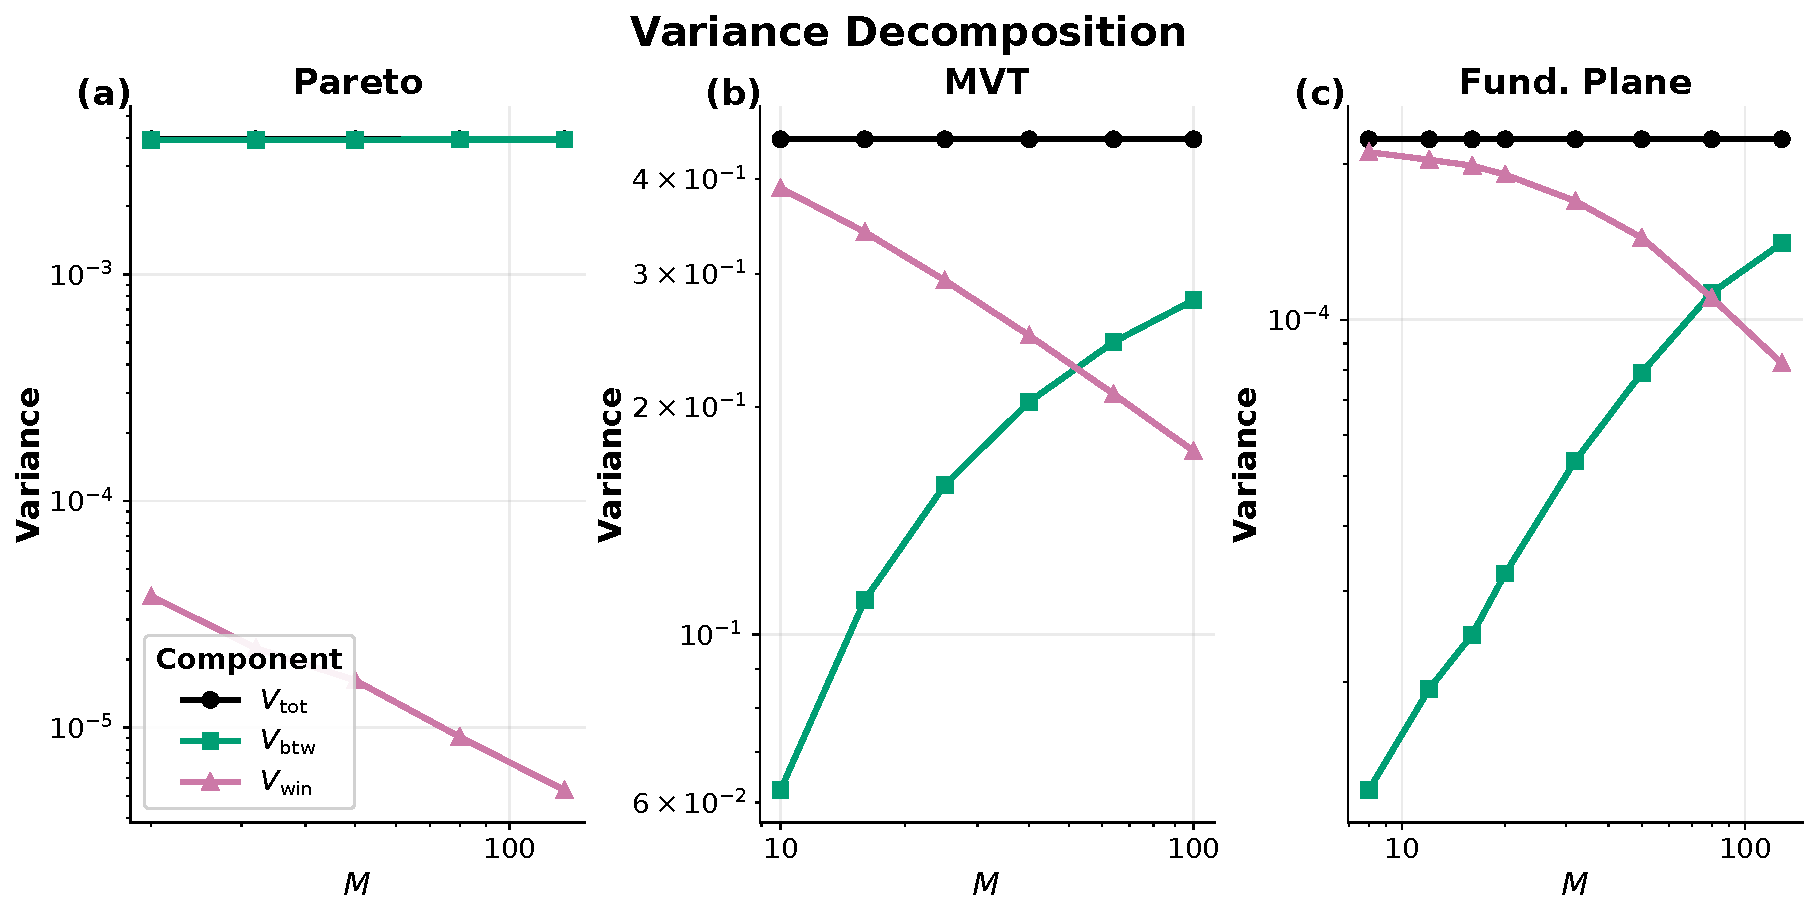
\includegraphics[width=\linewidth]{f3.pdf}
\caption{The variance decomposition eq. \eqref{eq:identity} is partition-invariant. Each panel shows the terms of \eqref{eq:identity}, averaged over the $S = 1000$ Monte Carlo draws. As the partition refines, the between-RF term $\Vcell$ (squares) rises and the within-RF term $\Vwithin$ (triangles) falls, while their sum $\Vtotal$ (circles) is constant in $M$. Estimands: (a) the Pareto shape parameter; (b) the MVT degrees of freedom $\nu$; (c) the FP coefficient $a$. In (a), $\Vcell$ overplots $\Vtotal$, with $\Vwithin$ more than two orders of magnitude smaller.}
\label{fig:invariance}
\end{figure}

The estimator variances shown in Figure~\ref{fig:invariance} are similar to those identified by the standard bootstrap, which is reported in Figure~\ref{fig:coverage}(a), broken out by estimand. The paired ratio $\log(V_{\mathrm{QIJ}}/V_{\mathrm{boot}})$ conveys agreement (=0) or disagreement ($\pm$0) of QIJ's estimated sampling variance, compared to that of the standard bootstrap. Offsets of order $1/N$ are expected, since QIJ omits higher-order terms and the bootstrap carries its own $O(1/N)$ bias.
Figure~\ref{fig:coverage}(b) compares nominal and empirical coverage of the two interval estimators; QIJ tracks the unity slope, whereas standard bootstrap is mildly conservative at low nominal levels; at commonly used levels (0.90 and above) both methods are nominal within Monte Carlo error (gray shaded band). Figure~\ref{fig:coverage}(c) compares mean interval widths from both methods at the nominal level at which each method attains 95\% empirical coverage (0.955 for QIJ, 0.949 for the bootstrap): the width ratios lie between 1.004 and 1.065, largest for the two tail-probability estimands.

\begin{figure}[t]
\centering
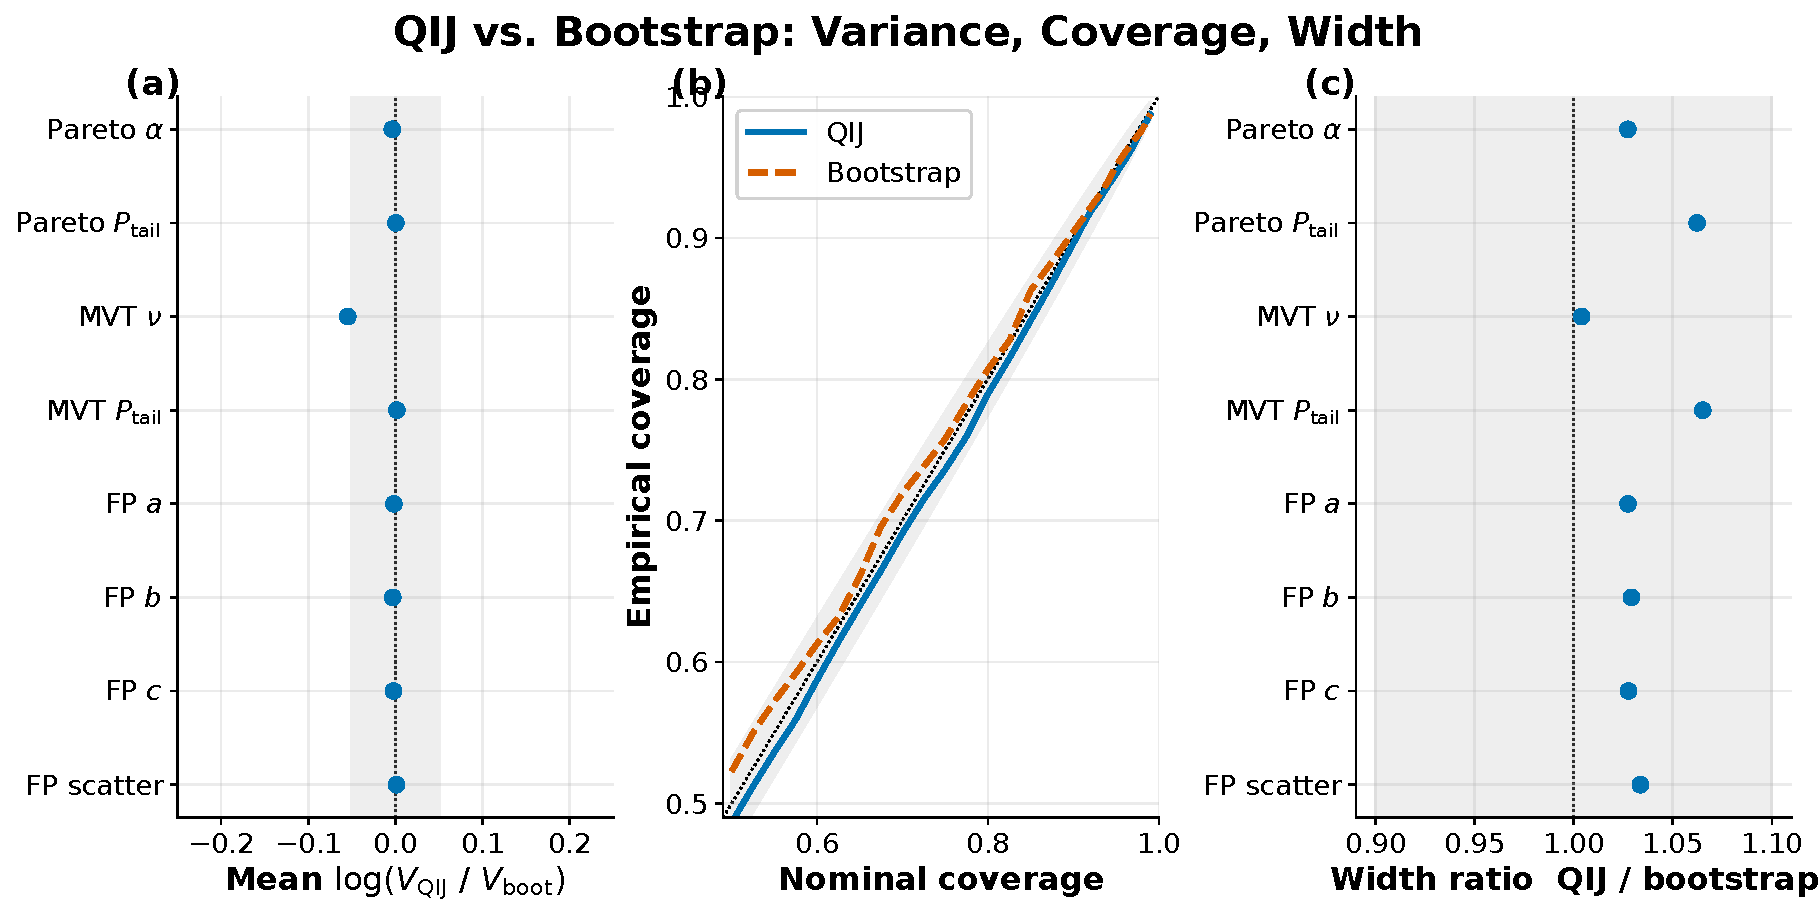
\includegraphics[width=\linewidth]{f2.pdf}
\caption{Validation against the standard bootstrap. (a) Mean $\log(V_{\mathrm{QIJ}}/V_{\mathrm{boot}})$ per estimand, with 95\% CI whiskers (smaller than the markers at $S = 1000$); the shaded band marks $\pm 0.05$. All estimands fall inside the band except the MVT $\nu$, just outside at $-0.055$. (b) Empirical versus nominal coverage, pooled over all datasets and estimands, with the $\pm 1.96\sqrt{p(1-p)/S}$ Monte Carlo band: QIJ tracks the diagonal across the level grid; the bootstrap is mildly conservative at low nominal levels, and both are nominal at common levels (e.g, 90\%, 95\%, 99\%). (c) Mean interval width ratios, QIJ over bootstrap, evaluated at the nominal level where each method attains 95\% empirical coverage (0.955 for QIJ, 0.949 for the bootstrap); the shaded band marks $\pm 10\%$. Ratios range from 1.004 to 1.065, largest for the tail-probability estimands.}
\label{fig:coverage}
\end{figure}

\subsection{The Computation-Accuracy Frontier}\label{sec:res-compute}

To produce the intervals presented in Figure~\ref{fig:coverage}, QIJ demands only $M{+}1$ evaluations of estimator $T$; compared to the standard bootstrap, which requires hundreds-thousands, this can be considerably cheaper. To demonstrate this compute cost savings, Figure~\ref{fig:compute} traces what an incremental evaluation of $T$ buys both methods (in terms of interval width) when estimating the $\sigma$ (velocity dispersion) slope of the galaxy fundamental plane data. As presented here, QIJ utilized $M = 50$ prototypes (for 51 evaluations of $T$) to achieve the same width that the standard bootstrap achieves around boot replicate $B \sim$1800 (the figure shows all widths relative to that computed from standard bootstrap's width after 2,000 boot replicates). Both methods estimate the same interval around FP's population quantity $a$; QIJ achieves widths comparable to standard boot, but with far fewer (51 $<<$ $\sim$1800) estimator evaluations. 

\begin{figure}[t]
\centering
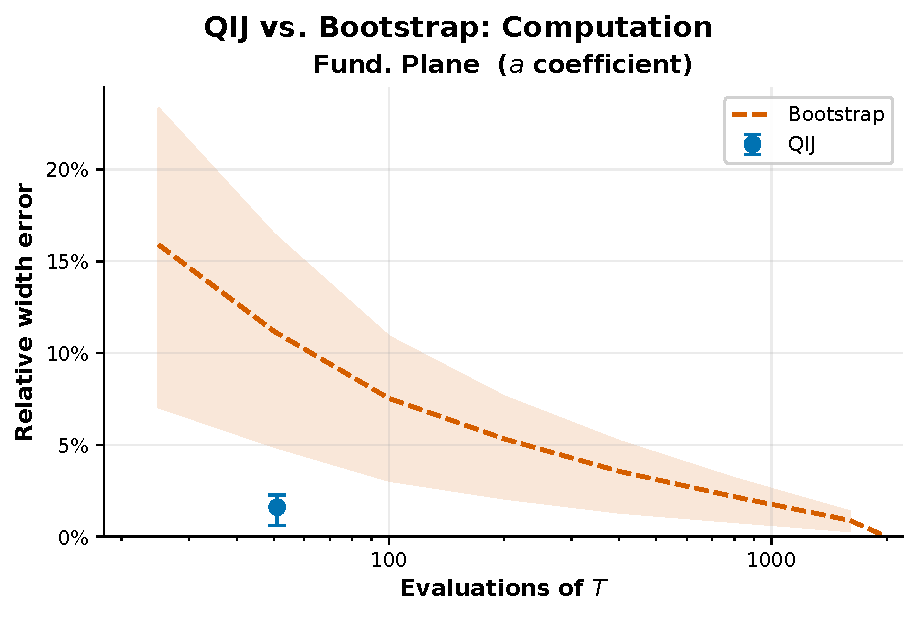
\includegraphics[width=.85\linewidth]{f7.pdf}
\caption{Computation frontier on the FP coefficient $a$. For each bootstrap replicate, the bootstrap 95\% interval width is recomputed from its first $b$ replicates (in sequence) and then compared to the full $B = 2000$ reference (dashed line: mean over the $S = 1000$ Monte Carlo draws; ribbon: interquartile range); the error at $b = B$ is zero by construction. The QIJ point shows the width of QIJ's deterministic interval at $M{+}1 = 51$ evaluations against the same converged bootstrap reference (whiskers: interquartile range); QIJ's width is partition-invariant (Fig.~\ref{fig:invariance}), so a single operating point suffices. Standard bootstrap does not achieve the width of QIJ intervals until replicate ~1800 (cumulatively requiring ~1800 estimator evaluations).}
\label{fig:compute}
\end{figure}

% ======================================================================
\section{Conclusions}\label{sec:conclusions}
% ======================================================================

A fitted vector quantizer supports nonparametric interval estimation. The route is not resampling through the partition, which draws its randomness from precisely the variability the quantizer minimized, but perturbation across it: the RF counts fluctuate with exactly known covariance, the estimator's sensitivity to each count costs one evaluation, and $M{+}1$ deterministic evaluations therefore replace $B$ resamples. An exact identity keeps the accounting honest: the within-RF term that QIJ's perturbations cannot detect is computed rather than assumed, and the partition-invariance of the total provides a built-in correctness test. On three testbeds, including a real astronomical problem with empirically known truth, QIJ delivers nominal coverage at bootstrap-matched widths, at a small fraction of the computation.

The identity invites questions beyond parity that we develop in companion work: what the omitted term itself measures (its decay with $M$ turns out to carry the effective dimension of the data), and how a quantizer should be fitted when the goal is inference rather than distortion. Extending the multinomial engine to survey weights and dependent data, and shrinkage across RFs using prototype-adjacency structure, are further steps toward inference on real catalogues.

\begin{credits}
\subsubsection{\ackname} JT and SSRO acknowledge support from NSF AAG 2107942, NASA ADAP 80NSSC23K0476, and the US NSF under Cooperative Agreement 2421782 and the Simons Foundation grant MPS-AI-00010515 awarded to the NSF-Simons AI Institute for Cosmic Origins --- CosmicAI, \url{https://www.cosmicai.org/}. SSRO also acknowledges support from a Peter O'Donnell Distinguished Researcher Fellowship and a Donald Harrington Fellowship.
\subsubsection{\discintname} The authors have no competing interests to declare that are relevant to the content of this article. \todo{confirm disclosure wording}
\end{credits}

\bibliographystyle{splncs04}
\bibliography{refs}

\end{document}
